% !TEX root = thesis.tex
\chapter{深層学習のアルゴリズム}
Deep Learningは、多層ニューラルネットワーク(MLP)のうち、普通隠れ層が2つ以上のものをいう。2006年にHintonらによって、このようなDeepな構造を学習させる方法が発見され、発展への道が開けた\cite{hinton2006a-fast, hinton2006reducing}。従来よりも多くのレイヤーを扱うことで、より複雑な関数を学習できるようになった。Deep Learningは、数々の分類タスクにて、従来手法を大きくしのぐ成果を収め、注目を浴びている。例えば第1章で触れたように、2012年には、GoogleがYoutubeビデオの静止画を使って多層ニューラルネットワークの教師なし学習を行わせ、結果として、猫を認識するユニットや人を認識するユニットを学習させることに成功したと共に、ImageNet Large Scale Visual Recognition Competition(ILSVRC)というデータセット\cite{deng2009imagenet:}の分類にて、state of the artの結果を残した。この章では、Deep Learningで使われているアルゴリズムの詳細について述べる。
\section{Deep Belief Network}
最初にMLPの学習のブレイクスルーとなったのは、2006年のHintonらによるDeep Belief Nets(DBN)\cite{hinton2006a-fast, hinton2006reducing}である。このモデルについて解説する。
\subsection{unsupervised pretrainingとfinetuning}
この研究では、MLPの重みをランダムに初期化した後、すぐバックプロパゲーション学習にかけるのではなく、各レイヤーの重みをあらかじめ教師無し(unsupervised)学習で調整して、隠れ層が効率の良い素性を学習できるよう仕込んでおくというアイデアが使われた。この事前学習のことを、pretrainingと呼び、バックプロパゲーションにて学習する段階の方は、finetuningと呼ぶ。pretrainingの段階では、入力側から1レイヤーずつ学習を行い、学習済のレイヤーは固定して動かさない(Greedy Layer-wise pretraining)。finetuningの段階では、全てのレイヤーをバックプロパゲーションにて同時に変化させていく。\par
unsupervised pretrainingをどのような基準で行うかが問題だが、この研究では、Restricted Boltzman Machine(以下RBM)というモデルを用いている。RBMとは、ニューラルネットワークの一種で、可視変数層と隠れ変数層の2つのレイヤーから成り立っている。DBNにおいては、可視変数=入力データと考えておけばよい。RBMモデルの学習を進めることで、入力データ→隠れ変数への推論モデルを得ることができる。これがDeep Learningの最大の特徴の1つである、「抽象度の高い素性への変換方法自体を学習する」ことに対応している。DBNでは、RBMを1レイヤーずつ学習させながら、RBM同士を「前のレイヤーの隠れ層 = 次のレイヤーの入力層」となるようにつなげていく。これにより「入力層→抽象度の低いレイヤー→...→抽象度の高いレイヤー→出力」という、複数の隠れ層をもつDeepな構造を作り、上手くpretrainingさせることに成功している。RBMを積み重ねた最も上のレイヤーに、普通の線形レイヤーを1つ置いて、「最も抽象度の高い素性→出力値」の推測を行わせることが多い。なお、finetuningにおけるバックプロパゲーションでは、RBMにあった「隠れ層→入力層」の方のつながりは、最終レイヤーにおける誤差に影響しない。よって、以前からあるfeed-forwardなMLPと同様に学習させることができる。
\subsection{Restricted Boltzman Machine}
DBNのpretrainingに用いられるRestricted Boltzman Machine\cite{smolensky1986information}とは、ニューラルネットワークを用いた生成モデルの一種である。まず生成モデルについて説明する。\par
クラス分類問題を確率的アプローチで解く方法は、生成モデル(generative model)と識別モデル(判別モデル、discriminative model)の2つに大別できる\cite{bishop2006pattern}\footnote{確率モデルを介さず、入力からクラスを得る識別関数を直接導くことも出来る。}。クラス分類問題では、まずクラス事後確率$p(C_k|x)$を各クラス$k$に対して求める。基本的には入力$x$に対して最もクラス事後確率が大きくなったクラスに分類することになる\footnote{医療における誤診断など、誤分類のタイプに応じて重要度が異なる場合、損失関数(loss function)を導入することもある。}。識別モデルでは、クラス事後確率$p(C_k|x)$のみを直接学習するのに対し、生成モデルでは、まずクラスの条件付き密度$p(x|C_k)$を学習する。これと、別途求めたクラスの事前確率$p(C_k)$を用いることで、クラス事後確率は
\begin{equation}
p(C_k|x) = \frac{p(x | C_k)p(C_k)}{p(x)} = \frac{p(x | C_k)p(C_k)}{\sum_{k}p(x | C_k)p(C_k)}
\end{equation}
によって求められる。これは、入力とクラスの同時確率$p(C_k, x)$を求めることと等価である。生成モデルの利点は、クラス分類のモデルだけでなく、入力データの性質に関する情報をも同時に得られる点にある。しかし、一般に識別モデルよりも複雑で困難な問題を解く必要が生じるため、常に生成モデルが用いられるわけではない。\par
さて、前述したように、RBMは可視層と隠れ層の2レイヤーで構成されるニューラルネットワークである。入力層の各ユニットの値を$v_j$, 隠れ層の各ユニットの値を$h_i$とおく。これらをまとめたベクトルをそれぞれ$\bm{v}=\{v_1, v_2, ...\}, \bm{h}=\{h_1, h_2, ...\}$とおく。これは、例えば$\bm{v}$が画像や音声などの入力データをベクトル化したもので、$\bm{h}$がこれらの変数の関係を説明する変数だと考えれば良い。ただし、$\bm{h}$が即$\bm{v}$のクラス分類に対応するとは限らないことに注意する。RBMの学習を進めると、$p(\bm{v}|\bm{h})$と$p(\bm{h}|\bm{v})$との、2方向の条件付き確率のモデルが同時に得られる。\par
RBMの学習は、自由エネルギーと呼ばれる従属変数を最小にするように行われる\footnote{自由エネルギーという呼び名は、物理学から採られている。}。ここでは、最も簡単かつ重要な、$v_j, h_i\epsilon\{0,1\}$のケースについて述べる。Wをvとhの間の重み、bとcを、それぞれvとhに対応するバイアス項とする。このとき、RBMにおける自由エネルギー$F(v)$は、
\begin{equation}
F(v) = -b' v-\sum_{i}log(1+e^{(c_i+W_{i}v)})
\end{equation}
となる。この自由エネルギーを、SGDなどのアルゴリズムを用いて最小化することで、目標となる生成モデルを得ることができる。なお、自由エネルギーの導入と最小化というアプローチは、Energy-Based Modelと呼ばれるアルゴリズム群に共通して用いられる概念であり、自由エネルギーにはさらに一般的な定義が存在するが、割愛する。
\subsection{DBNの成果}
この研究では、評価実験としてMNISTの手書き数字認識データセットを用いている。彼らは各レイヤーのユニット数が"784-500-500-2000-10"という構造のDBNによって、学習を行った。そして、Permutation invariantと呼ばれるタスクにて、当時のstate fo the artを塗り替えたことにより、注目された。ここで、Permutation invariantとは、データを単なる1次元の値の集まりと見なし、2次元の画像という事前情報の利用を禁止した状態で、分類実験を行うことである。具体的には、画像的変形による水増しや、2次元的畳み込み(Convolutional Layerの節にて詳述)などが当てはまる。Permutation invariantの制約下で良い成果を出したDBNは、画像の性質を利用したConvolutional Netに比べたとき、画像以外の1次元のデータに対しても適用しやすいアルゴリズムだと考えられる。

%Deep Learningの登場 Hinton, Bengio, LeCun
%画像認識タスクでの成績、音声認識タスクでの成果、猫認識
%MNIST, CIFAR, SVHNなどにおけるconv.net、Maxout, DropConnectの優位

\section{深層学習モデルのバリエーションと詳細}
この節では、Deep Learningのアルゴリズムが、どのような要素の組み合わせで出来ているのか、紹介する。2章の最後で紹介した多層パーセプトロン(MLP)に、どのような工夫を加えることで学習が可能になったのか、使われている技術を列挙する。
%\subsection{pretraningとfinetuning}

\subsubsection{Multi Layer Perceptron (MLP)}
後述するMaxout Networkでは、単純なMLP構造を用いながら、いくつかのテクニックによって精度良い学習を実現している。
\subsubsection{}
(MLP, SDA, DBM, CNN)

\subsection{Dropoutとrobustnessの確保}
\label{c3_dropout}
Dropoutとは、2012年にHinton氏らによって提案された、過学習を防ぐための技術である\cite{hinton2012improving}。過学習とは、機械学習全般において使われる用語で、学習モデルが訓練中に見たデータへの適応を重視し過ぎたために、未知のデータをうまく識別できなくなる現象のことを指す。Dropoutでは、過学習を防ぐため、各レイヤーからの出力をランダムに消去してしまう。これによって各ユニットには、他のユニットに頼らず自力で学習をする必要が生じ、より様々な入力に対応しやすい堅固(robust)なモデルが獲得される、と考えられている。\par
DropConnectは、Dropoutをさらに一般化した手法である。DropConnectでは、各ユニットからの出力ではなく、ユニット同士のつながりをランダムにカットしている。図\ref{c3_dropconnect}は、DropConnectの著者による紹介Webページ\footnote{\url{http://cs.nyu.edu/~wanli/dropc/}}に掲載されている画像の引用である。ニューラルネットワークにおけるニューロン同士の接続が、ランダムに切断されている様子を表している。
\begin{figure}[tbp]
 \begin{center}
  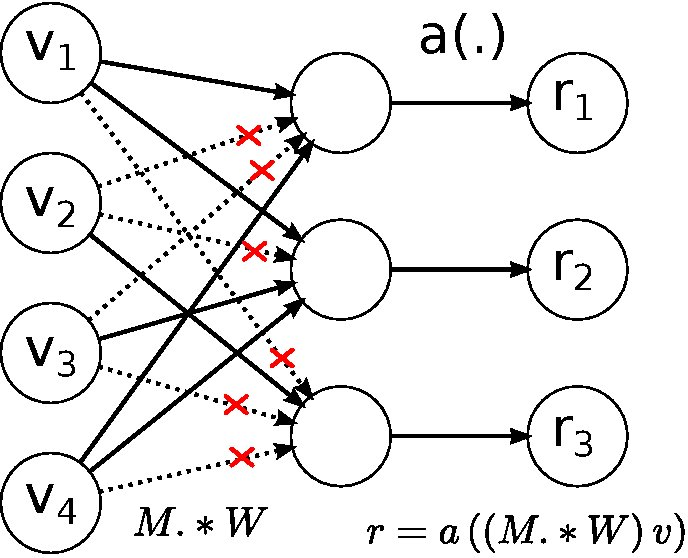
\includegraphics[width=50mm]{img/c3/nn_dc}
 \end{center}
 \caption{DropConnectの模式図}
 \label{c3_dropconnect}
\end{figure}
\subsection{活性化関数}
各ユニットに入力された値は、ある一定の関数によって増幅・変換される。これは人間の神経細胞を真似た仕組みで、神経細胞の化学物質による活性化にちなんで、活性化関数(activation function)と呼ばれる。この項では、ニューラルネットにおける様々な活性化関数を紹介する。
\subsubsection{sigmoidとhyperbolic tangent}
シグモイド関数は、以下の式で表される。
%\begin{equation}

%\end{equation}
\subsubsection{rectifier}
\subsubsection{Maxout Unit}
Maxout Networkとは、バックプロパゲーションを伴う単純な多層MLP構造に、\ref{c3_dropout}で述べたDropout法を組み合わせ、さらにMaxout Unitという特殊な活性化関数を併用したニューラルネットワークである\cite{goodfellow2013maxout}。Maxout Networkの1レイヤー分の構造を、図\ref{c3_maxout_arch}に示す。\par
Maxout Unitでは、複数の線形ユニットの出力について、maxを取っている。これにより、任意の凸関数を近似することが出来る。図\ref{c3_maxout_app}は、Maxout Unitが凸関数を近似する様子を、1次元の入力について示している。そして、複数のmaxout unitの線形和を取ることは、複数の近似された凸関数の線形和を取ることである。これによって、最終的に任意の連続関数を近似できることが証明されている。
\begin{figure}[tbp]
 \begin{center}
  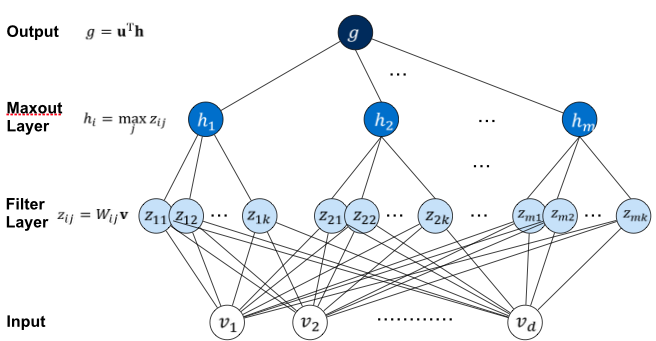
\includegraphics[width=100mm]{img/c3/maxout_arch}
 \end{center}
 \caption{Maxout Networkの構造図}
 \label{c3_maxout_arch}
\end{figure}
\begin{figure}[tbp]
 \begin{center}
  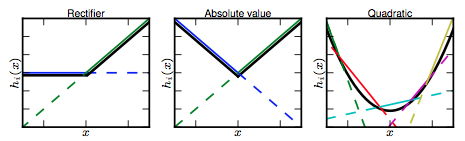
\includegraphics[width=100mm]{img/c3/maxout_app}
 \end{center}
 \caption{Maxout Unitが凸関数を近似する様子(1次元の場合)}
 \label{c3_maxout_app}
\end{figure}
